\documentclass[12pt,a4paper]{article}
\usepackage[utf8]{inputenc}
\usepackage[margin=1in]{geometry}
\usepackage{graphicx}
\usepackage{float}
\usepackage{amsmath}
\usepackage{listings}
\usepackage{xcolor}
\usepackage{enumitem}

% Code listing style
\lstset{
    language=C++,
    basicstyle=\ttfamily\footnotesize,
    keywordstyle=\color{blue},
    commentstyle=\color{green},
    stringstyle=\color{red},
    numbers=left,
    numberstyle=\tiny,
    frame=single,
    breaklines=true
}

\begin{document}

% Front Page
\begin{titlepage}
  \centering
  \vspace*{3cm}

  {\Huge\bfseries CSE 406 – Lab Report 9: FIFO Page Replacement Algorithm \par}
  \vspace{2.5cm}

  \noindent
  \begin{minipage}[t]{0.48\textwidth}
    {\large\bfseries Submitted By:}\\[0.5em]
    \Large
    Sharif Md. Yousuf \\
    ID: 22101128 \\
    Section: C-2 \\
    4th Year, 1st Semester \\
    Spring 2025
  \end{minipage}
  \hfill
  \begin{minipage}[t]{0.48\textwidth}
    {\large\bfseries Submitted To:}\\[0.5em]
    \Large
    Atia Rahman Orthi \\
    Lecturer \\
    Department of Computer Science \& Engineering \\
    University of Asia Pacific
  \end{minipage}

  \vfill

  {\Large\bfseries Date of Submission:} \\[0.5em]
  {\LARGE\bfseries 03 October, 2025 (Friday)}

  \vspace*{2cm}
\end{titlepage}

\section{Problem Statement}
In this lab, I was tasked with implementing a page replacement simulator using the FIFO (First In First Out) algorithm. The challenge was to create a program that, given a fixed number of frames and a sequence of page references, would simulate the process of loading pages into memory and replacing them when necessary. My program needed to track page hits and page faults, display the frame status at each step, and calculate performance metrics including hit ratio and fault ratio.

\subsection*{Input}
For my implementation, the program accepts:
\begin{itemize}
  \item Frame size (number of available frames in memory)
  \item Number of page references
  \item Sequence of page references
\end{itemize}

Here's an example of what I worked with:
\begin{verbatim}
Frame size: 3
Number of pages: 15
Page sequence: 7 0 1 2 0 3 0 4 2 3 0 3 2 1 2
\end{verbatim}

\subsection*{Output}
My program produces:
\begin{itemize}
  \item A detailed table showing page reference, frame status, and hit/miss for each step
  \item Total page requests
  \item Total page hits and page faults
  \item Hit ratio and fault ratio as percentages
\end{itemize}

\section{Objective}
Through this lab, I aimed to achieve several learning goals:
\begin{itemize}
    \item Gain a deep understanding of the FIFO page replacement algorithm
    \item Successfully implement FIFO to manage page frames using a queue data structure
    \item Learn how to track and visualize the state of memory frames at each page reference
    \item Calculate and analyze performance metrics including hit ratio and fault ratio
    \item Understand the concept of page faults and their impact on system performance
    \item Analyze the strengths and weaknesses of the FIFO approach to page replacement
\end{itemize}

\section{Source Code Screenshot}
\begin{figure}[H]
  \centering
  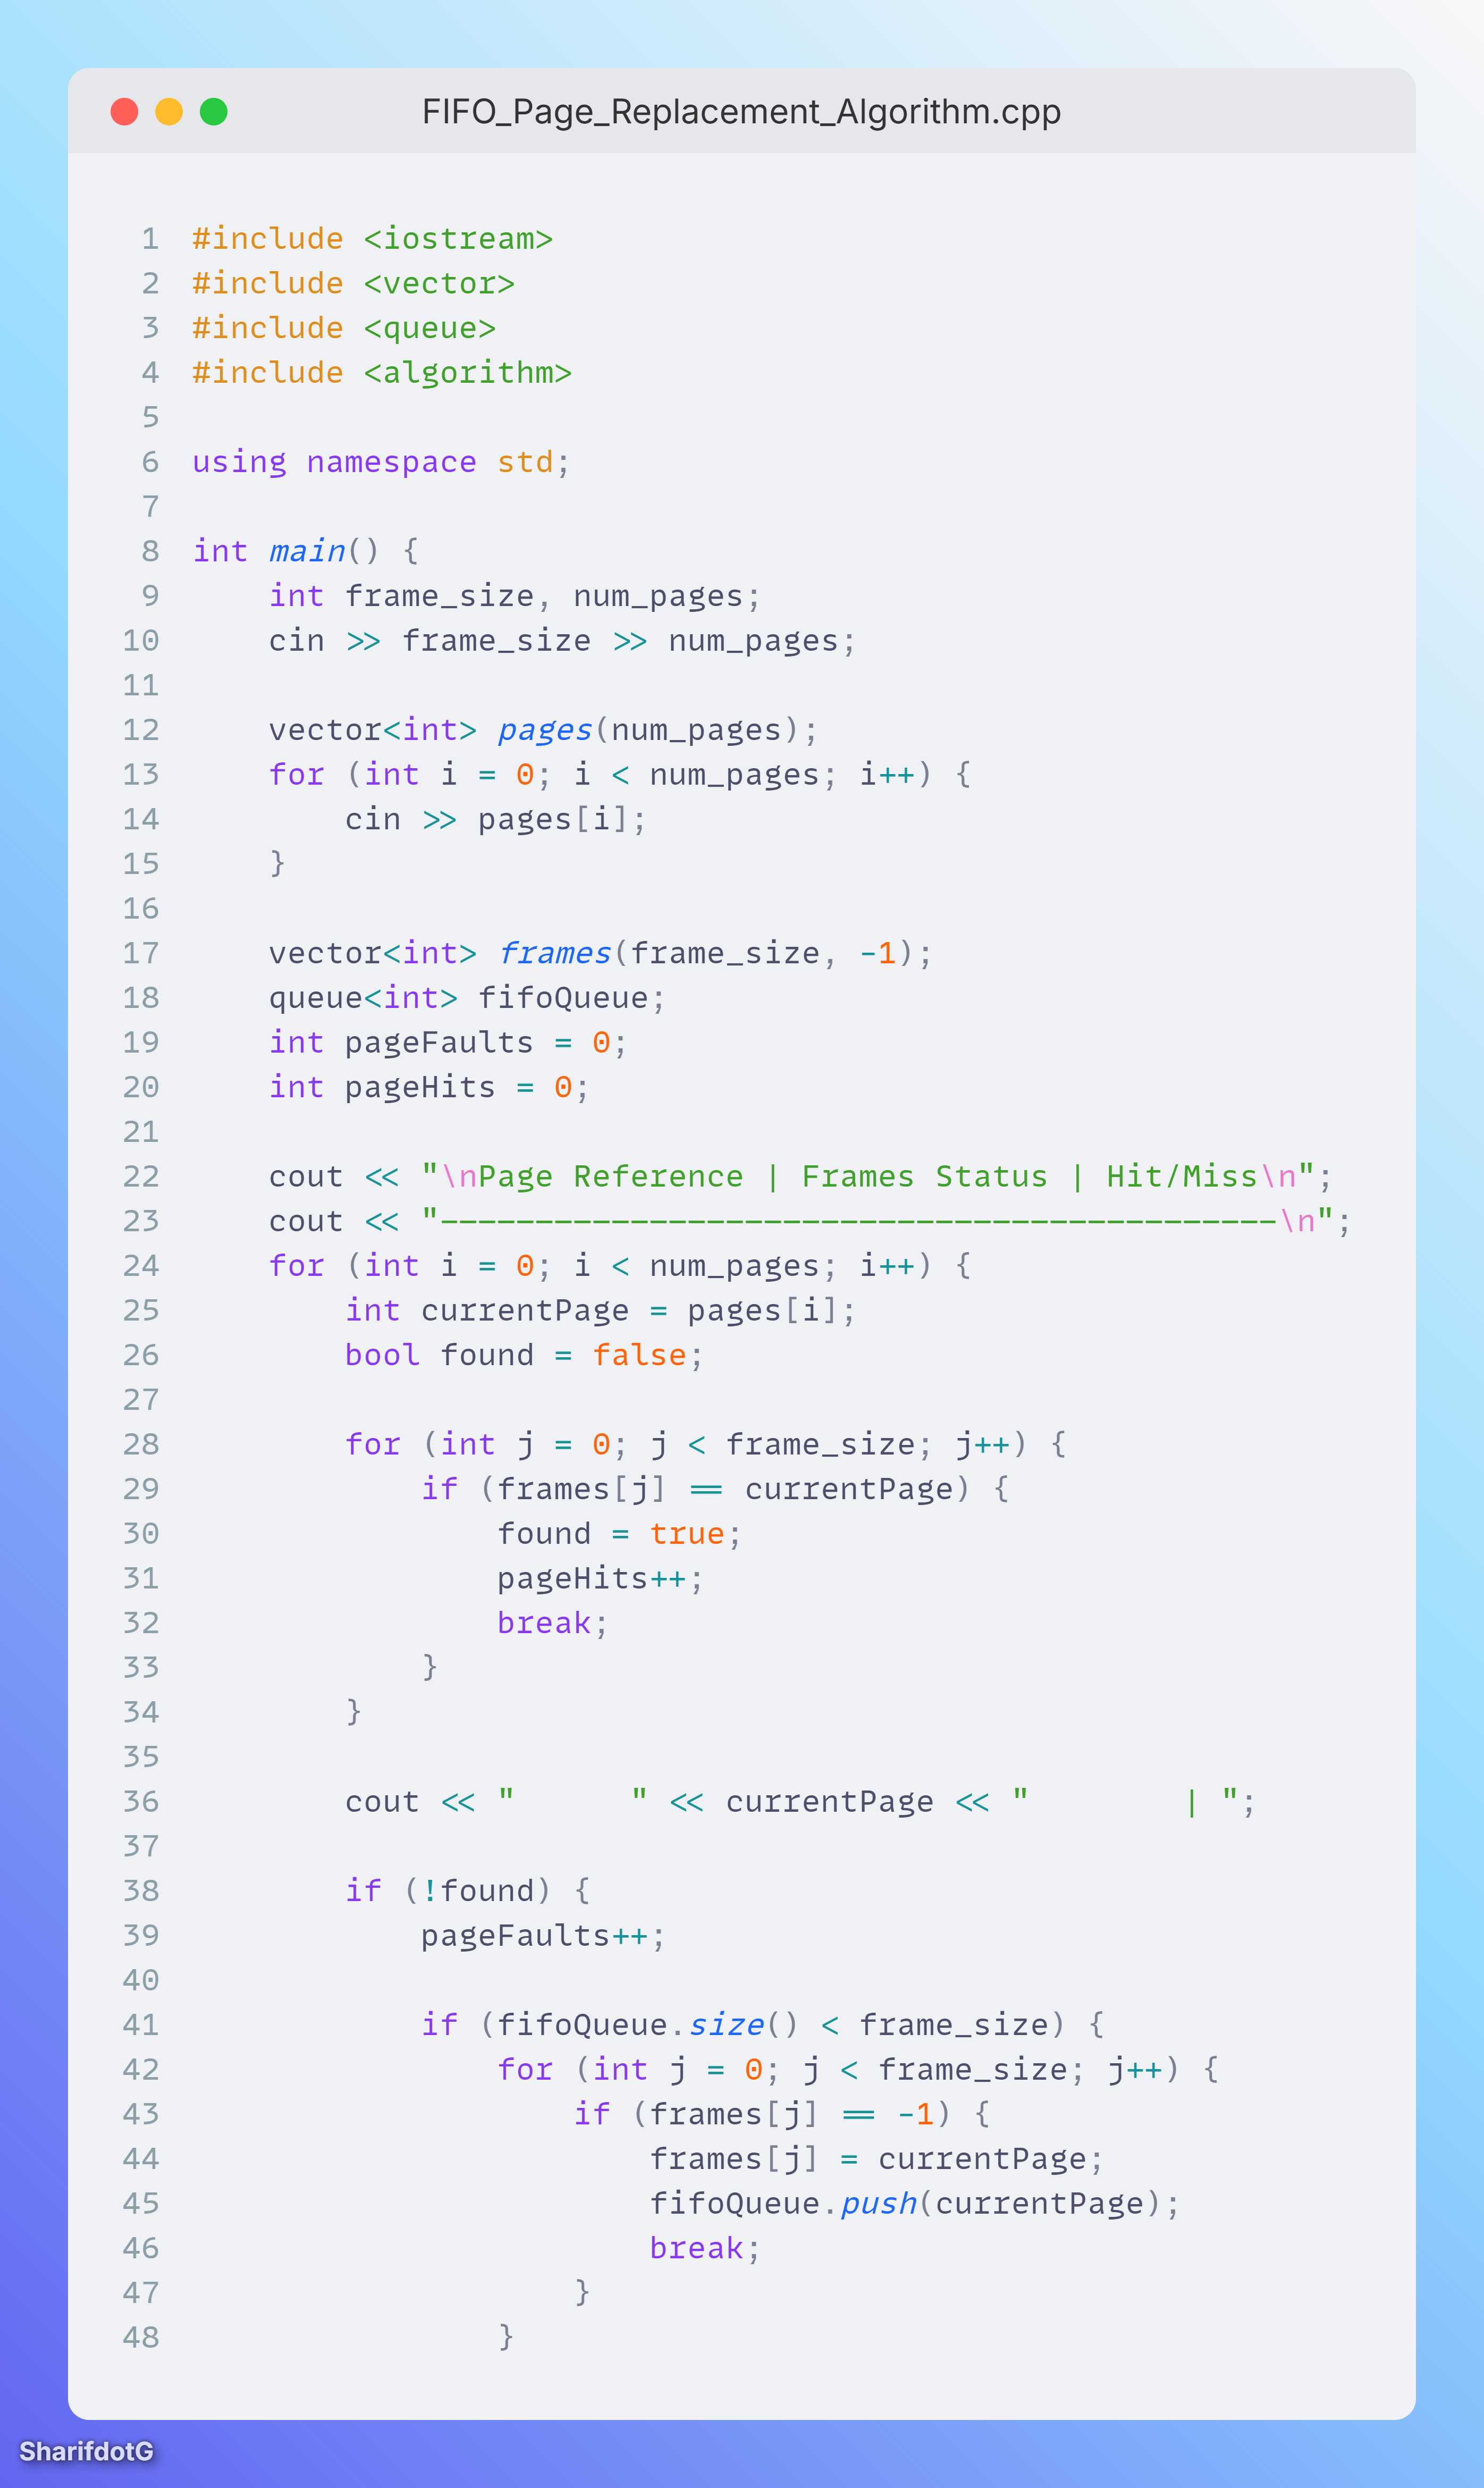
\includegraphics[width=0.75\textwidth]{Code1.png}
  \caption{FIFO Page Replacement Algorithm Source Code (Part 1)}
\end{figure}

\begin{figure}[H]
  \centering
  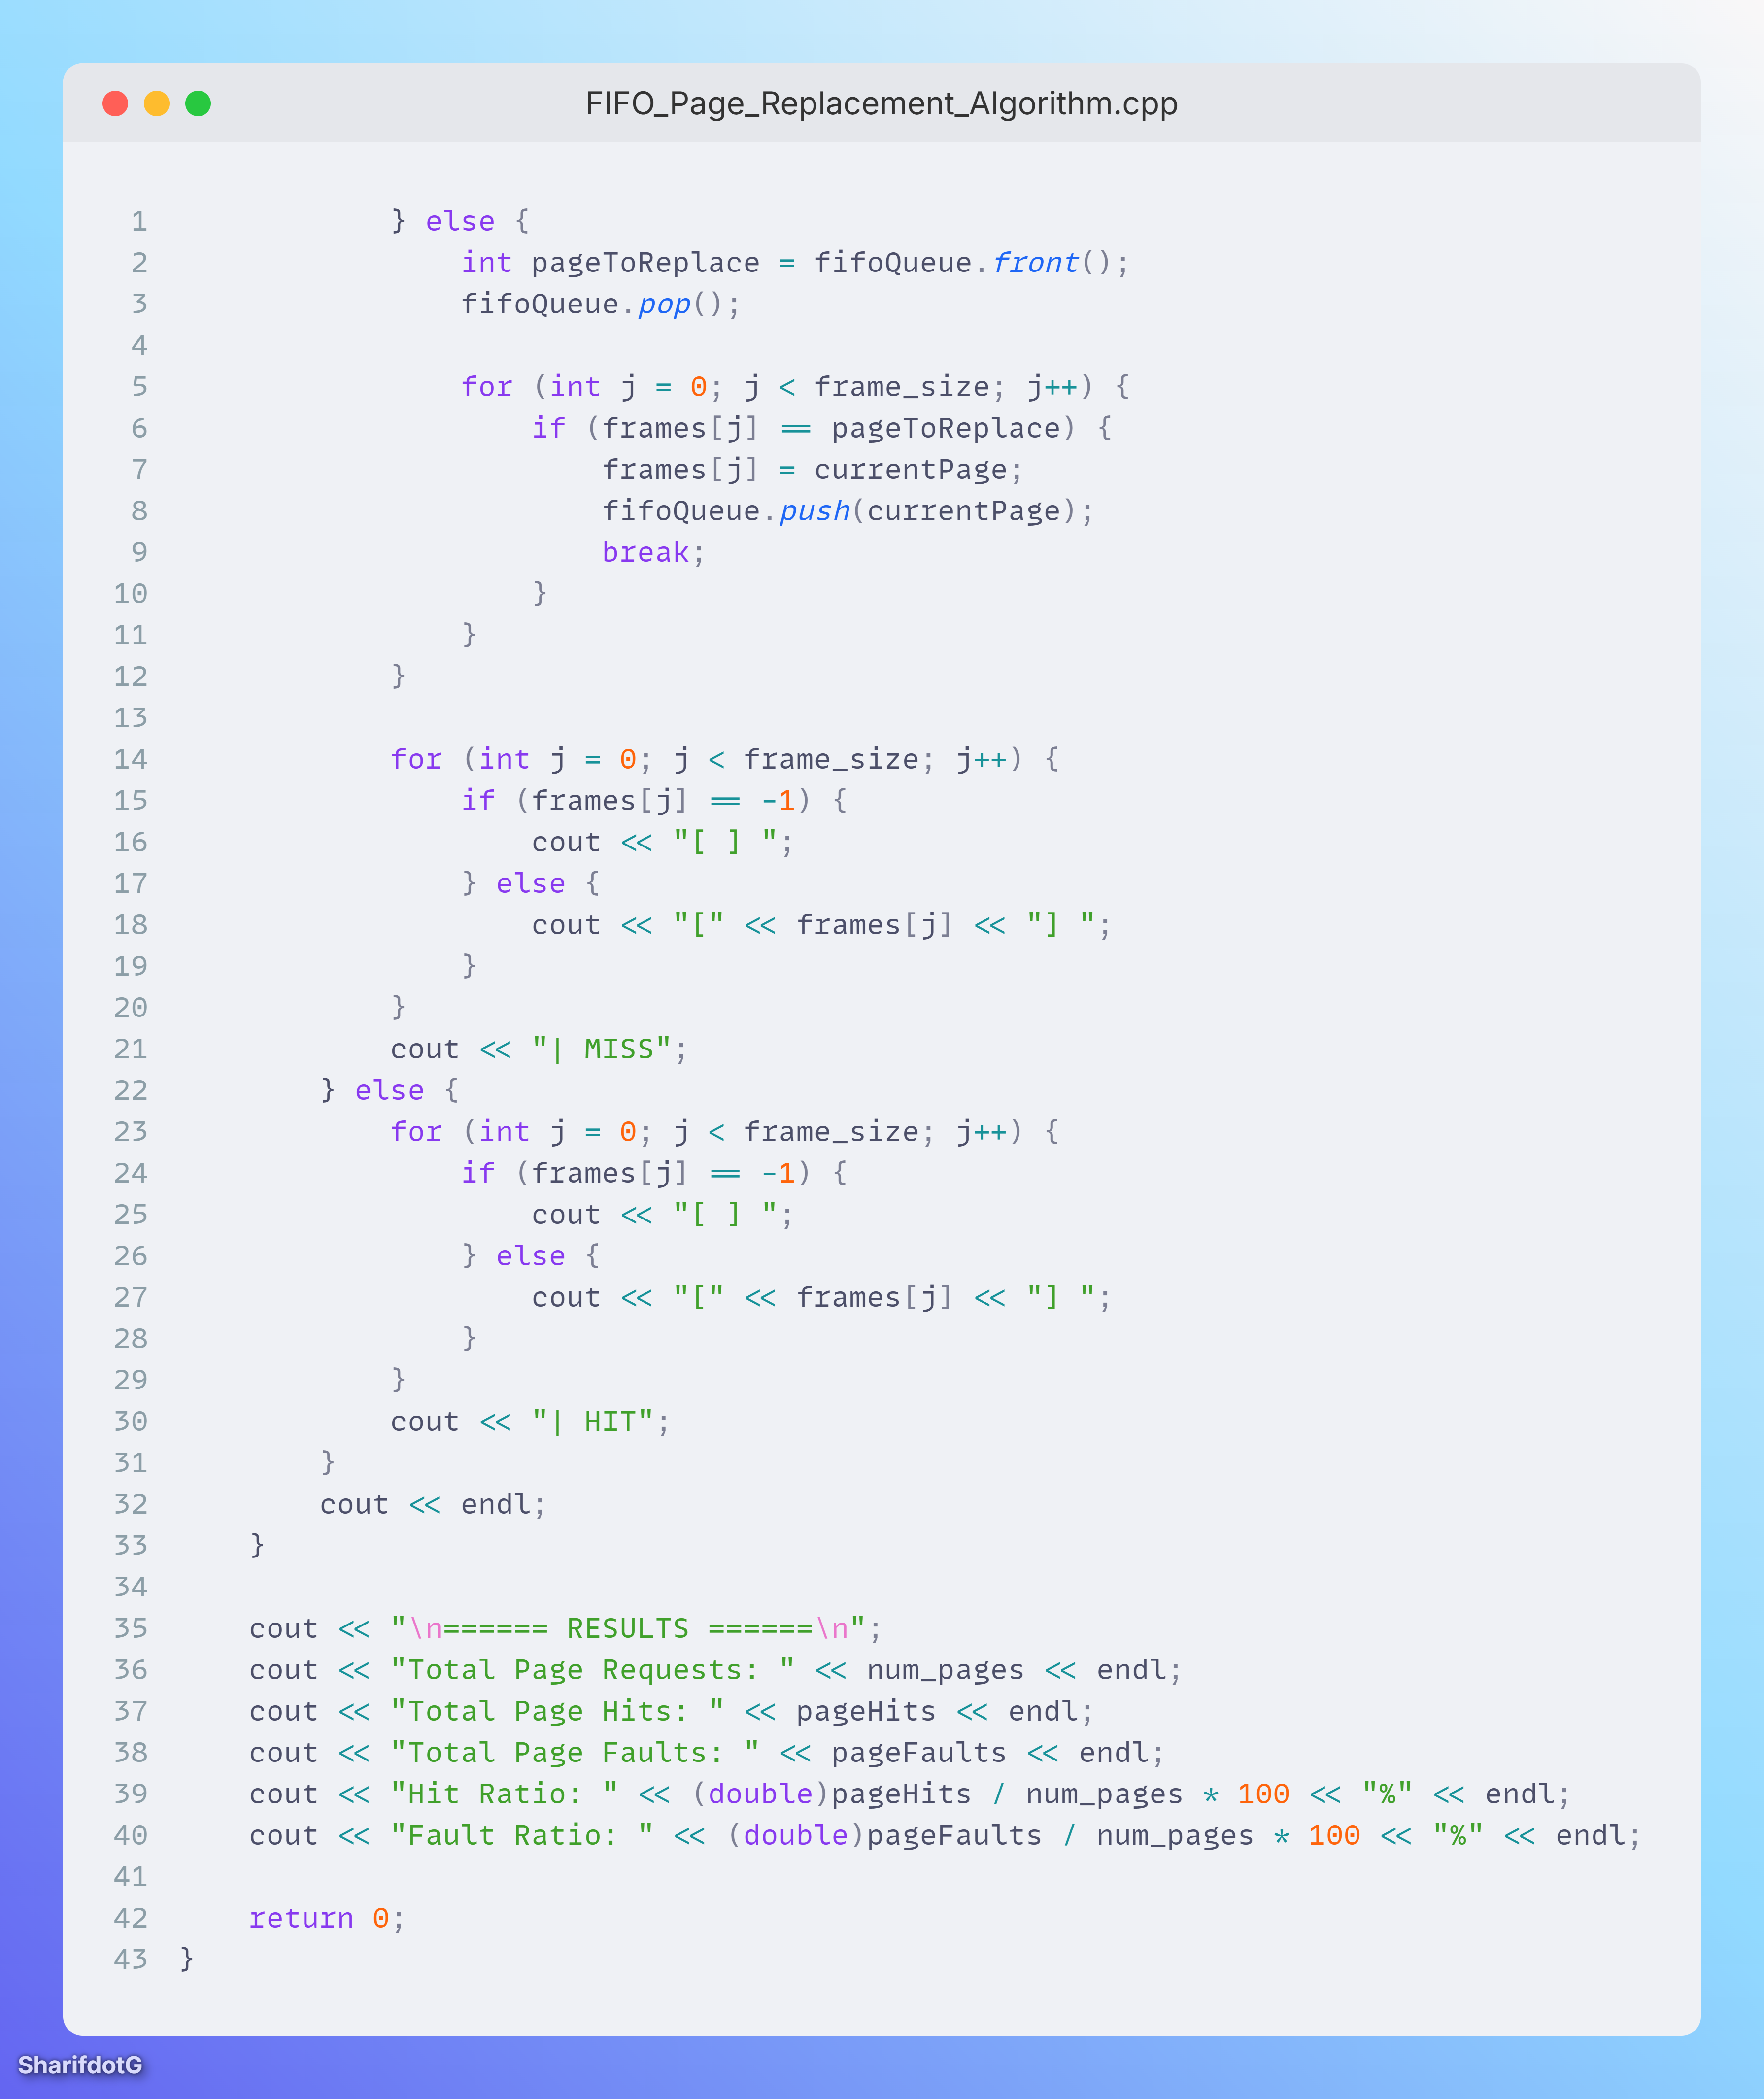
\includegraphics[width=0.75\textwidth]{Code2.png}
  \caption{FIFO Page Replacement Algorithm Source Code (Part 2)}
\end{figure}

\section{Output Screenshot}
\begin{figure}[H]
  \centering
  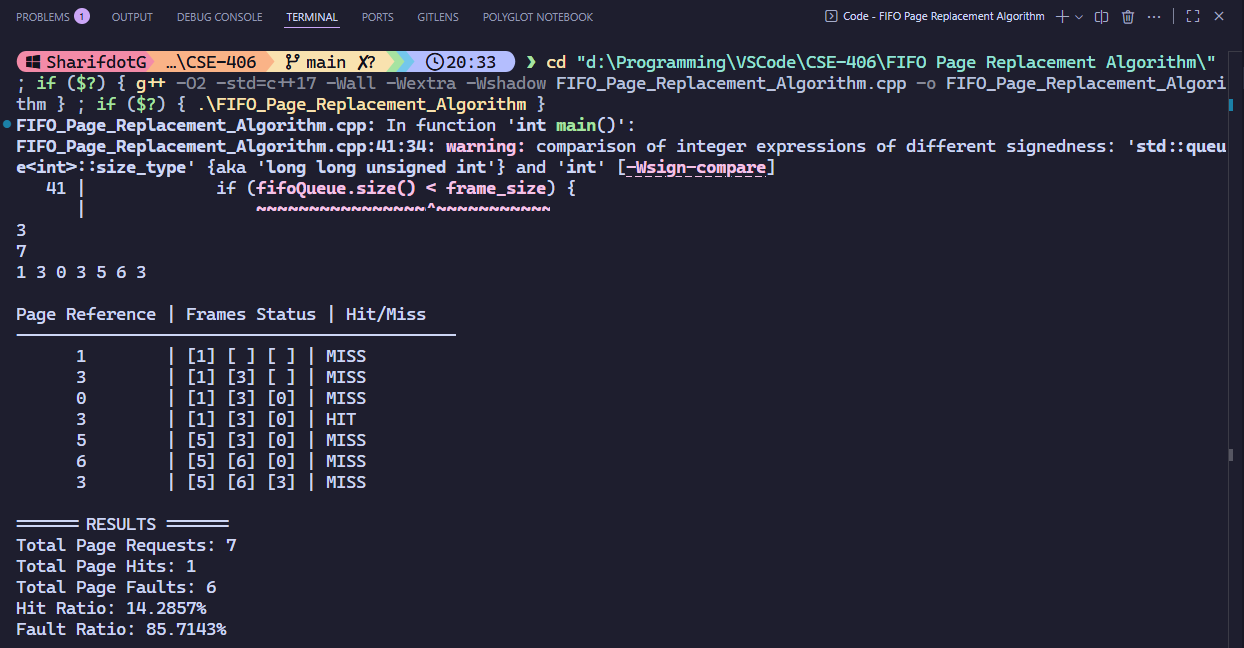
\includegraphics[width=0.85\textwidth]{Screenshot 2025-10-03 203502.png}
  \caption{FIFO Page Replacement Program Output}
\end{figure}

\section{Discussion}
Working with the FIFO page replacement algorithm has been an enlightening experience that introduced me to the fundamental concepts of memory management in operating systems. I discovered that FIFO represents one of the simplest approaches to page replacement, following the intuitive principle that the oldest page in memory should be replaced first. Here's what I learned about its key characteristics:

\begin{itemize}
    \item \textbf{Simplicity:} I found that FIFO's greatest strength is its straightforward implementation. Using a queue data structure, the algorithm naturally maintains the order in which pages entered memory, making replacement decisions trivial.
    \item \textbf{Queue-Based Management:} What I appreciated was how FIFO leverages the FIFO queue property perfectly - the page at the front of the queue is always the oldest and thus the first candidate for replacement.
    \item \textbf{Fair Replacement Policy:} I noticed that FIFO treats all pages equally, giving each page an equal opportunity to remain in memory based solely on arrival time, without considering usage patterns.
    \item \textbf{Performance Limitations:} However, I observed a significant drawback - FIFO doesn't consider page usage frequency or recency. A frequently used page that arrived early might be replaced, causing unnecessary page faults.
    \item \textbf{Belady's Anomaly:} Through my research, I learned that FIFO suffers from Belady's Anomaly, where increasing the number of frames can sometimes lead to more page faults rather than fewer.
\end{itemize}

\textbf{Performance Analysis:}
\begin{itemize}
    \item \textbf{Page Fault Rate:} I observed that FIFO's performance heavily depends on the page reference pattern. Sequential or repeated patterns can lead to higher fault rates if frequently used pages are replaced.
    \item \textbf{Predictability:} The algorithm provides predictable behavior, making it easy to analyze and debug, which is valuable for understanding memory management concepts.
    \item \textbf{Real-world Limitations:} I learned that while FIFO is rarely used alone in modern systems, it serves as a foundation for understanding more sophisticated algorithms like LRU and optimal page replacement.
\end{itemize}

Through this implementation, I gained insights into the trade-offs between simplicity and performance in algorithm design, understanding that FIFO's ease of implementation comes at the cost of optimal performance.

\section{Conclusion}
Completing this FIFO page replacement implementation has been a valuable educational experience that provided me with foundational knowledge of memory management in operating systems. Through this project, I've gained a clear understanding of how page replacement algorithms work and their critical role in virtual memory systems.

While I observed that FIFO may not provide optimal performance due to its ignorance of page usage patterns, I've learned that it serves as an important baseline for understanding more complex algorithms. The simplicity of FIFO makes it an excellent starting point for studying page replacement strategies, and its predictable behavior helps in grasping the fundamental concepts of page faults and memory management.

This lab has been invaluable in showing me how the design of memory management algorithms involves balancing simplicity, performance, and practical implementation considerations. Understanding FIFO's strengths and limitations will be essential as I explore more advanced page replacement algorithms like LRU, LFU, and optimal replacement in future studies. The hands-on experience with tracking hits, faults, and calculating performance metrics has prepared me well for analyzing and comparing different memory management strategies.

\end{document}
